\documentclass[12pt]{article}
\usepackage{tikz}
\usepackage{pgf-umlcd}
\begin{document}
\ \\
%
%%%%%%%%%%%%%%%%%%%%%%%%%%%%%
%
\section{Ecuaciones Diferenciales Exactas}
Para esta secci\'{o}n, partiremos del hecho de que la condici\'{o}n necesaria y 
suf\/iciente para que la expresi\'{o}n
\begin{equation}
P(x,y)dx+Q(x,y)dy 
\end{equation}
sea una diferencial exacta de alguna funci\'{o}n $F(x,y)$ es que
\begin{equation}
\frac{\partial P}{\partial y}=\frac{\partial Q}
{\partial x},
\label{Ecu77-1}
\end{equation}
donde esas derivadas parciales son funciones continuas.

%%%%%%%%%%%%%%%%%%%%%%%%%%%%%
%
Considere ahora la 
ecuaci\'{o}n %diferencial
\begin{equation}
P(x,y)dx+Q(x,y)dy=0,
\label{Ecu77-2}
\end{equation}
y suponga que las funciones 
$P(x,y)$ y $Q(x,y)$ satisfacen la condici\'{o}n 
(\ref{Ecu77-1}), por lo tanto, existe una funci\'{o}n 
$F(x,y)$ tal que
\begin{eqnarray}
dF&=&\frac{\partial F}{\partial x}dx+
\frac{\partial F}{\partial y}dy\\
&=&P(x,y)dx+Q(x,y)dy.
\end{eqnarray}
A una ecuaci\'{o}n diferencial as\'{i} se le conoce como ecuaci\'{o}n diferencial exacta.

%%%%%%%%%%%%%%%%%%%%%%%%%%%%%

Es claro que la funci\'{o}n 
\begin{equation}
 F(x,y)=C,
\end{equation}
donde $C$ es una constante arbitraria, ser\'{a} una soluci\'{o}n de la ecuaci\'{o}n (\ref{Ecu77-2}). 

%%%%%%%%%%%%%%%%%%%%%%%%%%%%%

\newpage
A continuaci\'{o}n, se obtendr\'{a} una forma expl\'{i}cita de la funci\'{o}n $F(x,y)$.

%%%%%%%%%%%%%%%%%%%%%%%%%%%%%

Por hip\'{o}tesis la condici\'{o}n (\ref{Ecu77-1}) se cumple, as\'{i} que podemos escribir
\begin{equation}
 \frac{\partial F}
 {\partial x}= P(x,y)
\mbox{\ \ \ y\ \ \ }
\frac{\partial F}{\partial y}=Q(x,y).
\label{Ecu77-3}
\end{equation}


%%%%%%%%%%%%%%%%%%%%%%%%%%%%%

Ahora, la primera de estas ecuaciones seguramente ser\'{a} satisfecha por la expresi\'{o}n
\begin{equation}
 F(x,y)=\int P(x,y)dx+f(y),
 \label{Ecu77-4}
\end{equation}
donde la $y$ que aparece bajo el signo de la integral es tratada como un par\'{a}metro y $f(y)$ es una funci\'{o}n arbitraria que solo depende de $y$.


%%%%%%%%%%%%%%%%%%%%%%%%%%%%%

Ahora se determinar\'{a} la funci\'{o}n $f(y)$, de tal manera que (\ref{Ecu77-4}) satisfaga la segunda de las ecuaciones ({\ref{Ecu77-3}).

%%%%%%%%%%%%%%%%%%%%%%%%%%%%%

Diferenciando (\ref{Ecu77-4}) con respecto a $y$ e igualando el resultado con $Q(x,y)$ se obtiene
\begin{equation}
\frac{\partial F}{\partial y}=
\frac{\partial}{\partial y}\int P(x,y)dx+
\frac{df}{dy}=Q(x,y),
\end{equation}

%%%%%%%%%%%%%%%%%%%%%%%%%%%%%

as\'{i} que
\begin{equation}
 \frac{df}{dy}=Q(x,y)-
\frac{\partial}{\partial y}\int P(x,y)dx.
\label{Ecu77-5}
\end{equation}

%%%%%%%%%%%%%%%%%%%%%%%%%%%%%

Por lo tanto,
\begin{equation}
 f(y)=\int\left[Q(x,y)-
\frac{\partial}{\partial y}\int P(x,y)dx\right]dy.
\label{Ecu77-6}
\end{equation}

%%%%%%%%%%%%%%%%%%%%%%%%%%%%%

Sustituyendo (\ref{Ecu77-6}) en (\ref{Ecu77-4}) nos conduce a la f\'{o}rmula expl\'{i}cita
\begin{equation}
 F(x,y)=\int P(x,y)dx+
\int\left[Q(x,y)-
\frac{\partial}{\partial y}\int P(x,y)dx\right]dy.
\label{Ecu77-7}
\end{equation}


%%%%%%%%%%%%%%%%%%%%%%%%%%%%%

\newpage

\section{Ejemplo}
Para ilustrar el uso de esta f\'{o}rmula, considere
\begin{equation}
 (2xy+1)dx+(x^{2}+4y)dy=0.
\end{equation}

%%%%%%%%%%%%%%%%%%%%%%%%%%%%%

Aqu\'{i}
\begin{equation}
 \frac{\partial P}{\partial y}=
\frac{\partial Q}{\partial x}=2x,
\end{equation}

%%%%%%%%%%%%%%%%%%%%%%%%%%%%%

as\'{i} que la f\'{o}rmula 
({\ref{Ecu77-7}) es aplicable.

%%%%%%%%%%%%%%%%%%%%%%%%%%%%%

Como ejercicio, COMPRUEBE que la sustituci\'{o}n de las expresiones $P(x,y)=2xy+1$ y $Q(x,y)=x^{2}+4y$ en la f\'{o}rmula (\ref{Ecu77-7}) da como resultado
\begin{equation}
 F(x,y)=x^{2}y+x+2y^{2}.
\end{equation}

%%%%%%%%%%%%%%%%%%%%%%%%%%%%%%

\section*{Lo que suele usarse}
En lugar de usar la f\'{o}rmula (\ref{Ecu77-7}), frecuentemente se procede como sigue:


%%%%%%%%%%%%%%%%%%%%%%%%%%%%%

Dado que $\partial P/\partial y=\partial Q/\partial x$, se sabe que existe una funci\'{o}n $F(x,y)$ tal que
\begin{equation}
 \frac{\partial F}{\partial x}=2xy+1
\mbox{,\ \ \ y\ \ }
\frac{\partial F}{\partial y}=x^{2}+4y
\end{equation}


%%%%%%%%%%%%%%%%%%%%%%%%%%%%%

Ahora, si integramos
\begin{equation}
 \frac{\partial F}{\partial x}=2xy+1
\end{equation}
Con respecto a $x$, tratando a $y$ como constante, resulta en
\begin{equation}
 F(x,y)=x^{2}y+x+c_{1}(y),
\end{equation}
donde $c_{1}(y)$ no es funci\'{o}n de $x$ pero podr\'{i}a ser una funci\'{o}n de $y$, dado que $y$ fue tratada como una constante.




%%%%%%%%%%%%%%%%%%%%%%%%%%%%%

Similarmente, la segunda condici\'{o}n
\begin{equation}
 \frac{\partial F}{\partial y}=x^{2}+4y,
\end{equation}


%%%%%%%%%%%%%%%%%%%%%%%%%%%%%

Integrando con respecto a $y$, da
\begin{equation}
 F(x,y)=x^{2}y+2y^{2}+c_{2}(x).
\end{equation}

%%%%%%%%%%%%%%%%%%%%%%%%%%%%%%

La comparaci\'{o}n de las dos expresiones para $F(x,y)$ muestra que si
\begin{equation}
 F(x,y)=x^{2}y+x+2y^{2},
\end{equation}

%%%%%%%%%%%%%%%%%%%%%%%%%%%%%%

entonces
\begin{equation}
 \frac{\partial F}{\partial x}=2xy+1
\mbox{\ \ \ \ y\ \ }
\frac{\partial F}{\partial y}=x^{2}+4y.
\end{equation}

%%%%%%%%%%%%%%%%%%%%%%%%%%%%%%%

Entonces, la soluci\'{o}n general de la ecuaci\'{o}n dada es
\begin{equation}
 x^{2}y+x+2y^{2}=C.
\end{equation}


%%%%%%%%%%%%%%%%%%%%%%%%%%%%%%%

\begin{center}
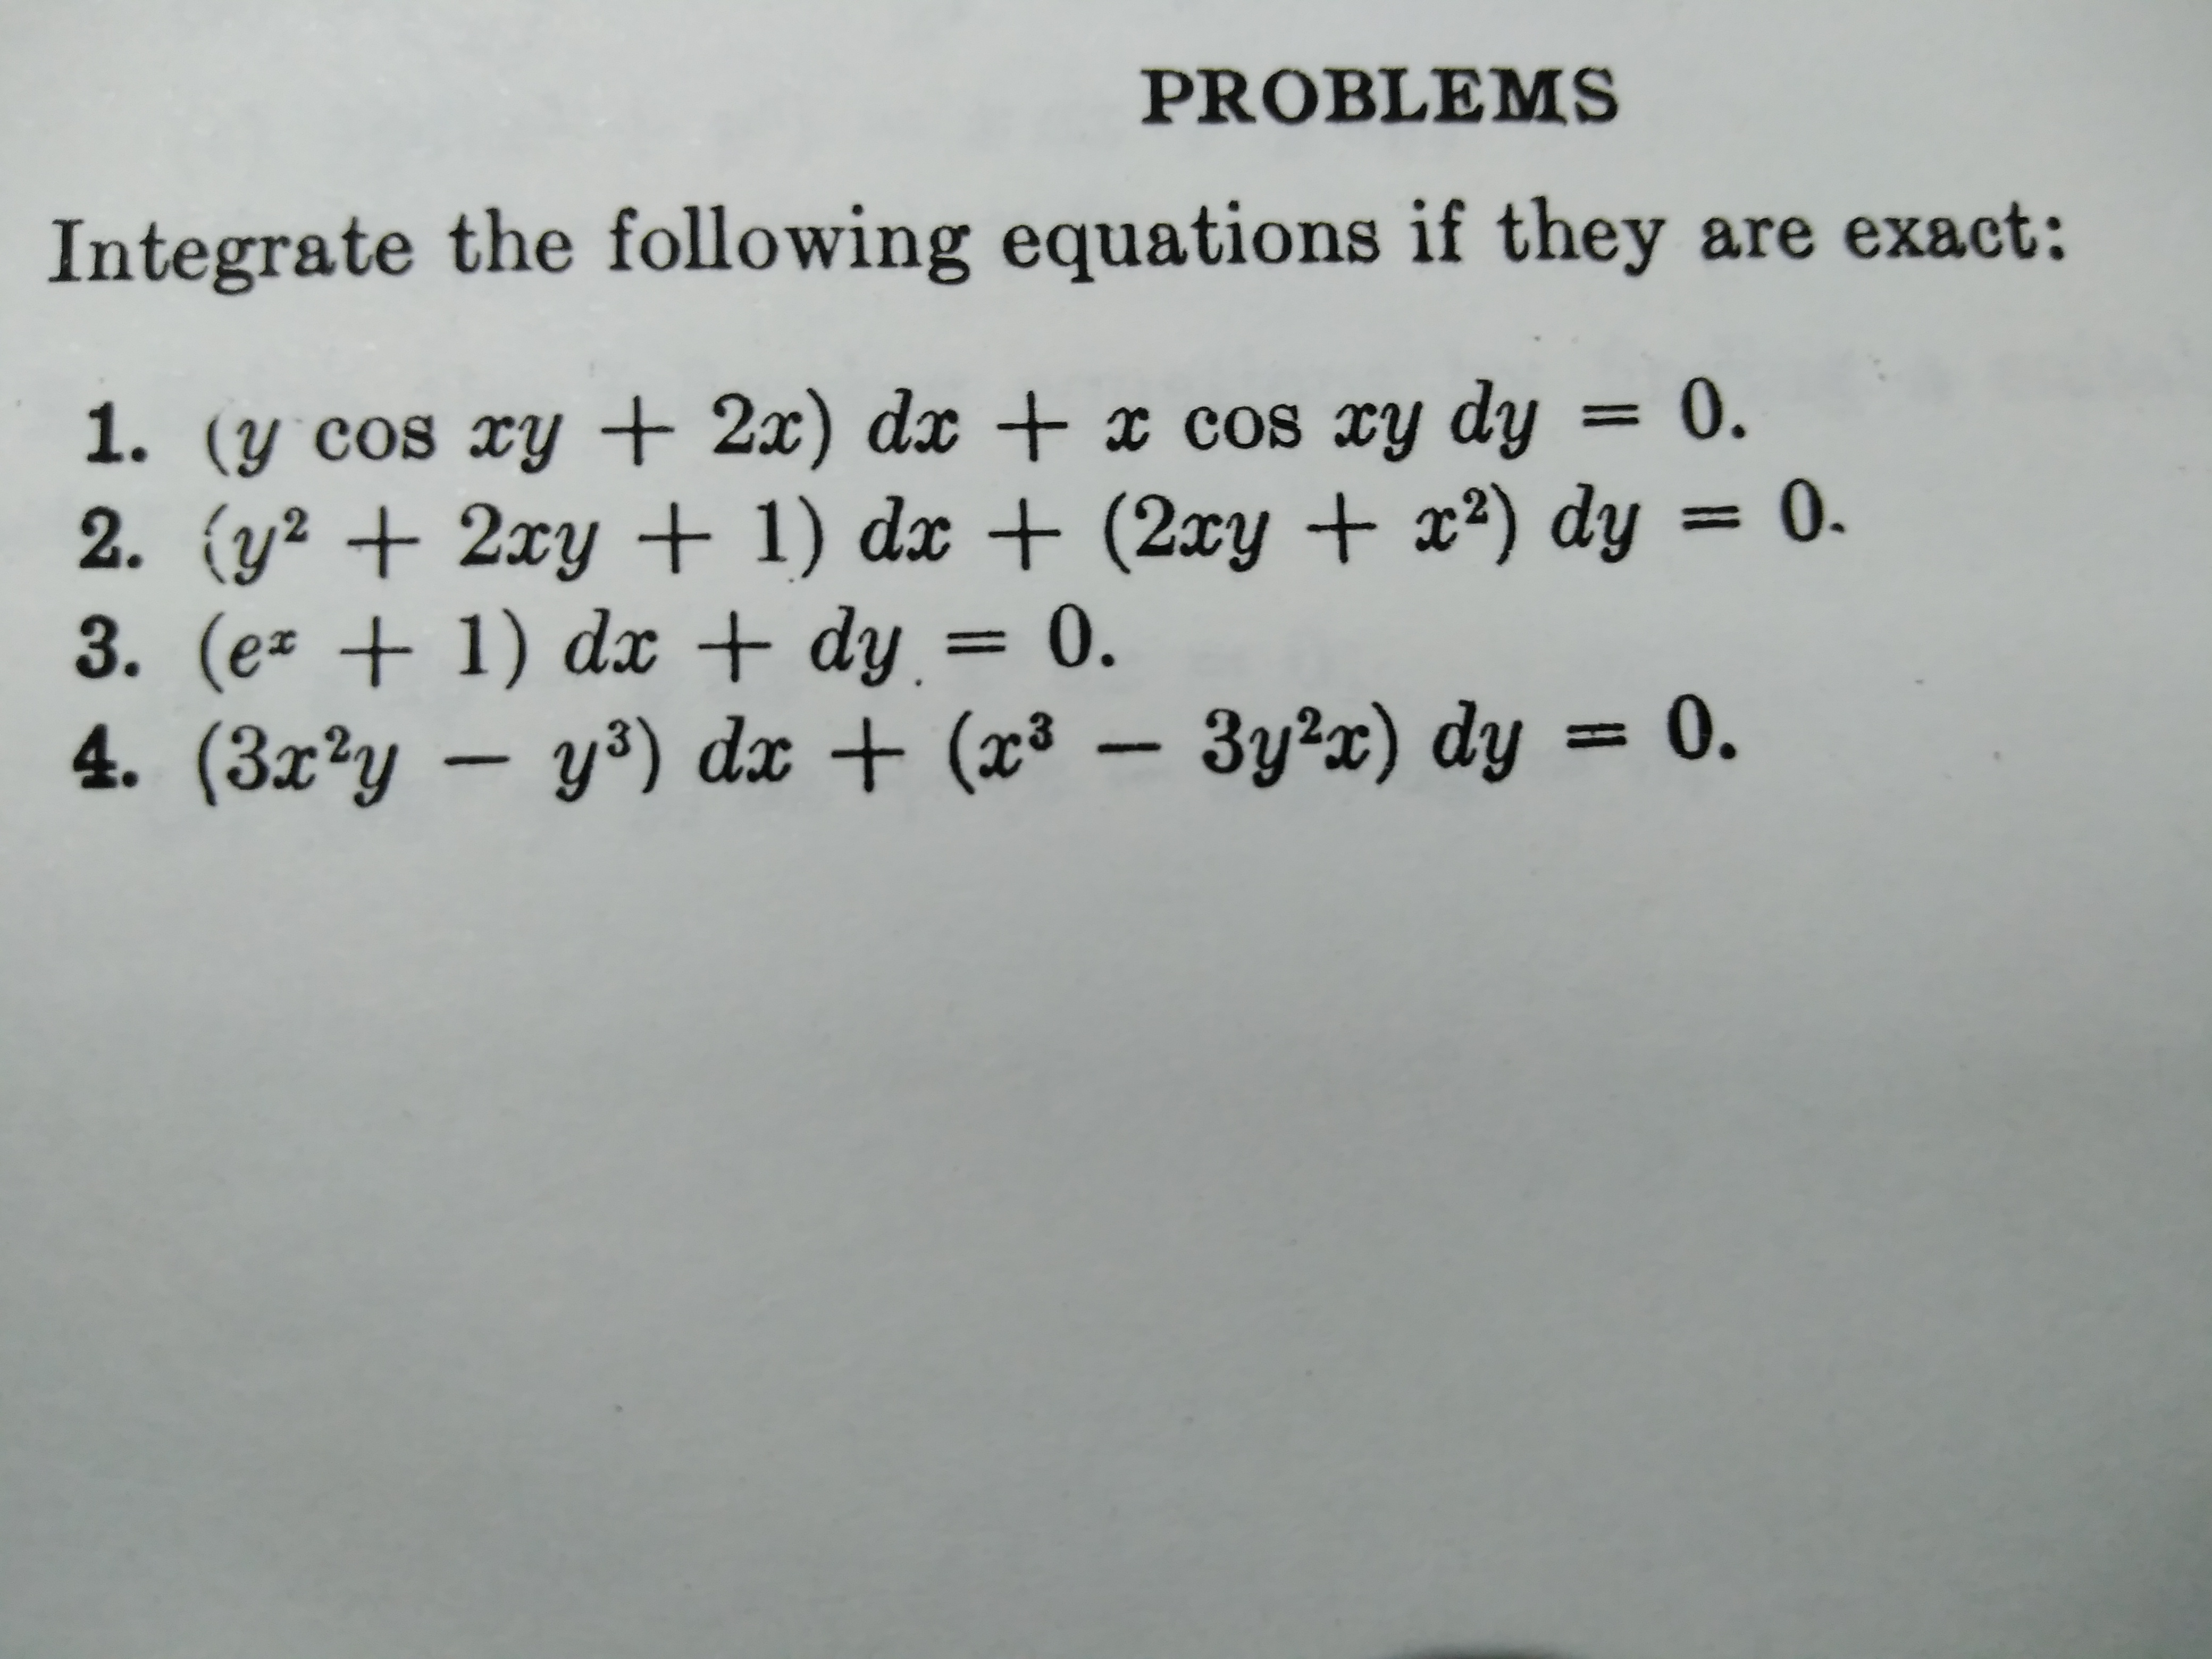
\includegraphics[width=12cm]{../images/Ecs_Exactas_1_a_4.jpg}
\end{center}
%%%%%%%%%%%%%%%%%%%%%%%%%%%%%
\begin{center}
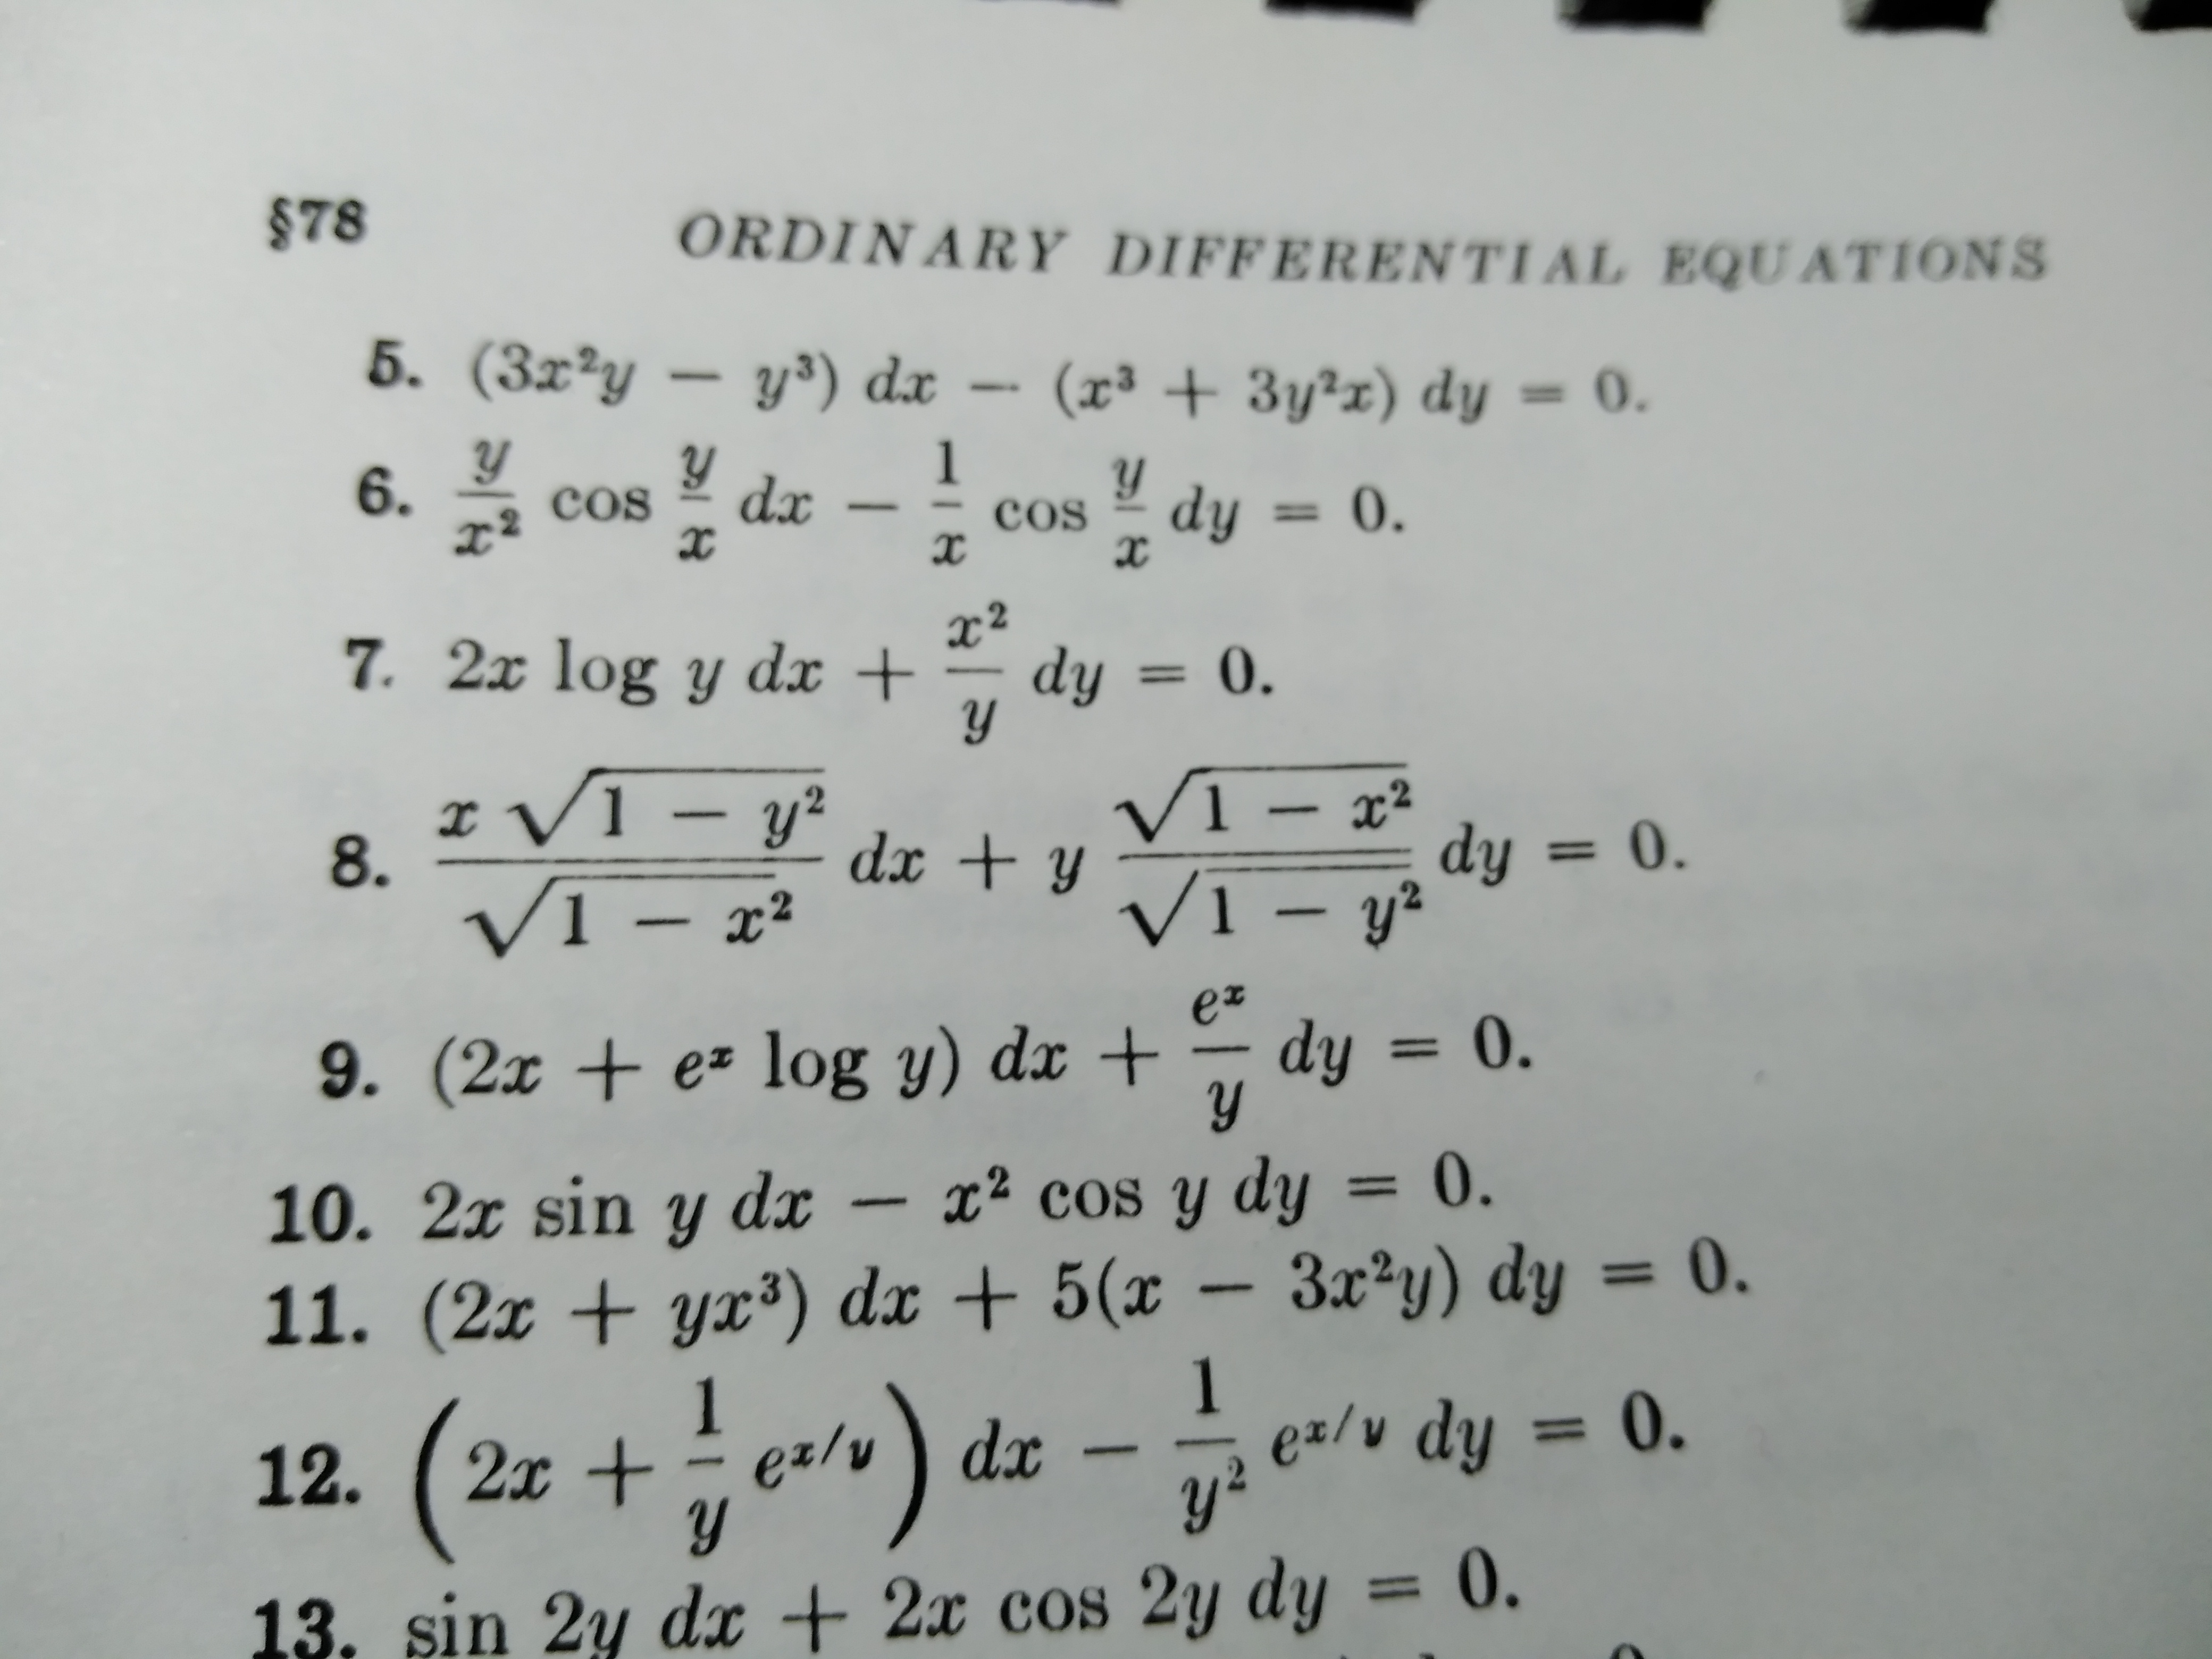
\includegraphics[width=12cm]{../images/Ecs_Exactas_5_a_10.jpg}
\end{center}


\end{document}
